\documentclass[12pt]{article}
\usepackage[pdfborder={0 0 0.5 [3 2]}]{hyperref}%
\usepackage[left=1in,right=1in,top=1in,bottom=1in]{geometry}%
\usepackage[shortalphabetic]{amsrefs}%
\usepackage{amsmath}
\usepackage{enumerate}
% \usepackage{enumitem}
\usepackage{amssymb}                
\usepackage{amsmath}                
\usepackage{amsfonts}
\usepackage{amsthm}
\usepackage{bbm}
\usepackage[table,xcdraw]{xcolor}
\usepackage{tikz}
\usepackage{float}
\usepackage{booktabs}
\usepackage{svg}
\usepackage{mathtools}
\usepackage{cool}
\usepackage{url}
\usepackage{graphicx,epsfig}
\usepackage{makecell}
\usepackage{array}

\def\noi{\noindent}
\def\T{{\mathbb T}}
\def\R{{\mathbb R}}
\def\N{{\mathbb N}}
\def\C{{\mathbb C}}
\def\Z{{\mathbb Z}}
\def\P{{\mathbb P}}
\def\E{{\mathbb E}}
\def\Q{\mathbb{Q}}
\def\ind{{\mathbb I}}

\DeclareMathOperator{\spn}{span}
\DeclareMathOperator{\ran}{ran}

\newtheorem{lemma}{Lemma}
\newtheorem{theorem}{Theorem}
\newtheorem{corollary}{Corollary}
\newtheorem{definition}{Definition}
\newtheorem{assumption}{Assumption}
\newtheorem{hypothesis}{Hypothesis}

\newtheorem{notation}{Notation}

\graphicspath{ {discrete/} }

\begin{document}

\section{Multipulses in Discrete Systems}

We want to look at Lin's method for multipulses in the discrete case. The model equation here is discrete NLS, but we want something more general since the result for dNLS is already known, at least if we are near the anticontinuum limit (Pelinovsky and Kevrekidis, 2005). The idea is that if we can find an appropriate generalization and setup for Lin's method, we can check it on dNLS.\\

\subsection{Discrete NLS}

Normalized form of dNLS is

\begin{equation}
i\dot{u}_n + \epsilon(u_{n+1} - 2 u_n + u_{n-1}) + |u_n|^2 u_n = 0
\end{equation}

the parameter $\epsilon$ represents the coupling between nodes, where the anticontinuum limit is given by $\epsilon = 0$. For this equation, we want to look for stationary solutions in a ``rotating'' frame, i.e. solutions of the form $\phi_n e^{i \omega t}$. To that end, we take $u_n \mapsto u_n e^{i \omega t}$ and simplify to get

\begin{equation}
i\dot{u}_n + \epsilon(u_{n+1} - 2 u_n + u_{n-1}) - \omega u_n + |u_n|^2 u_n = 0
\end{equation}

Stationary solutions then satisfy

\begin{equation}
\epsilon(u_{n+1} - 2 u_n + u_{n-1}) - \omega u_n + |u_n|^2 u_n = 0
\end{equation}

Before we continue, we let $u = v + i w$ and write dNLS as a two-dimensional system of equations by equating real and imaginary parts. For convenience, let $\Delta_2 u_n = (u_{n+1} - 2 u_n + u_{n-1})$. Then we have

\begin{align*}
\dot{v}_n &+ \epsilon \Delta_2 w_n - \omega w_n + v_n^2 w_n + w_n^3 = 0 \\
-\dot{w}_n &+ \epsilon \Delta_2 v_n - \omega v_n + v_n w_n^2 + v_n^3 = 0 \\
\end{align*}

$u_n = 0$ (i.e. $v_n = w_n = 0$) clearly satisfies this. For now, suppose we have a (real-valued) pulse solution $(q_n, 0)$. Taking the standard linearization ansatz

\[
\begin{pmatrix}v \\ w\end{pmatrix}_n = 
\begin{pmatrix}q \\ 0\end{pmatrix}_n + 
\eta \begin{pmatrix}a \\ b\end{pmatrix}_n e^{\lambda t}
\]

we obtain, upon substitution and simplification, the eigenvalue problem

\begin{align*}
L^+ a_n &= \omega a_n - \epsilon \Delta_2 a_n - 3 q_n^2 a_n = -\lambda b_n \\
L^- b_n &= \omega b_n - \epsilon \Delta_2 b_n - q_n^2 b_n = \lambda a_n
\end{align*}

We want to write this all as a difference equation. For that, we will need to expand to a fourth order system. Let $\tilde{a}_n = a_{n-1}$ and $\tilde{b}_n - b_{n-1}$. Substituting for $\Delta_2$, isolating the terms involving $n+1$, and dividing by $\epsilon$, we get

\begin{align*}
a_{n+1} &= \frac{1}{\epsilon}( \omega a_n - \epsilon (- 2 a_n + \tilde{a}_n) - 3 q_n^2 a_n + \lambda b_n ) \\
b_{n+1} &= \frac{1}{\epsilon}( \omega b_n - \epsilon (b_{n+1} - 2 b_n + \tilde{b}_n) - q_n^2 b_n - \lambda a_n )
\end{align*}

In matrix form, this is

\[
\begin{pmatrix}
a \\ \tilde{a} \\ b \\ \tilde{b}
\end{pmatrix}_{n+1} =
\frac{1}{\epsilon}
\begin{pmatrix}
\omega + 2 \epsilon - 3 q_n^2 & -\epsilon & \lambda & 0 \\
\epsilon & 0 & 0 & 0 \\
-\lambda & 0 & \omega + 2 \epsilon - q_n^2 & -\epsilon \\
0 & 0 & \epsilon & 0
\end{pmatrix}
\begin{pmatrix}
a \\ \tilde{a} \\ b \\ \tilde{b}
\end{pmatrix}_{n}
\]

which is of the form $V(n+1) = A(n; \omega, \lambda) V_n$, where $V = (a, \tilde{a}, b, \tilde{b})$. Since $q_n$ decays to 0 (exponentially) at both ends, $A(n; \omega, \lambda)$ decays (exponentially) to the asymptotic matrix $A_\infty(\omega, \lambda)$ at both ends.

\[
A_\infty(\omega, \lambda) = 
\frac{1}{\epsilon}
\begin{pmatrix}
\omega + 2 \epsilon & -\epsilon & \lambda & 0 \\
\epsilon & 0 & 0 & 0 \\
-\lambda & 0 & \omega + 2 \epsilon & -\epsilon \\
0 & 0 & \epsilon & 0
\end{pmatrix}
\]

For $\lambda = 0$, this becomes

\[
A_\infty(\omega, 0) = 
\begin{pmatrix}
\omega/\epsilon + 2 & -1 & 0 & 0 \\
1 & 0 & 0 & 0 \\
0 & 0 & \omega/\epsilon + 2 & -1\\
0 & 0 & 1 & 0
\end{pmatrix}
\]

Since this is block diagonal with idential blocks, the eigenvalues of this are 

\begin{align*}
\nu_{1,2} &= 1 + \frac{\omega}{2 \epsilon} \pm \frac{1}{2 \epsilon} \sqrt{\omega(4 \epsilon + \omega)} \\
&= 1 + \frac{\omega}{2 \epsilon} \left( 1 \pm \sqrt{1 + \frac{4 \epsilon}{\omega}} \right)
\end{align*}
each with algebraic multiplicity 2. For $\omega > 0$, since $\epsilon > 0$, we have $0 < \nu_1 < 1 < \nu_2$, i.e. $A_\infty(\omega, 0)$ is hyperbolic.\\

As in San98, we separate out the $\lambda$ stuff and write the eigenvalue problem as

\[
V_{n+1} = A(n; \omega, 0) V_n + \lambda B V_n
\]

where

\[
B = 
\begin{pmatrix}
0 & 0 & 1 & 0 \\
0 & 0 & 0 & 0 \\
-1 & 0 & 0 & 0 \\
0 & 0 & 0 & 0
\end{pmatrix}
\]

This looks good for Lin's method. Before we can do that, we need to know what is in the kernel of this. It is straightforward to see that $L^- q_n = 0$. By differentiating dNLS with respect to $\omega$, we also can see that $L^+ (-\partial_\omega q_n) = q_n$. Thus we should have an eigenvalue $\lambda = 0$ with algebraic multiplity 2 and geometric multiplicity 1. In other words, if we take $S = (0, 0, q, \tilde{q})^T$ and $T = (-\partial_\omega q, -\partial_\omega \tilde{q}, 0, 0)$, we have

\begin{align*}
S(n+1) &= A(n; \omega, 0) S(n) \\
T(n+1) &= A(n; \omega, 0) T(n) + B S(n)
\end{align*}

\subsection{Ablowitz-Ladik dNLS}

Here we look at Ablowitz-Ladik dNLS. The version we use is from Kapitula (2001).

\begin{equation}
i\dot{u}_n + \epsilon(u_{n+1} - 2 u_n + u_{n-1}) - \omega u_n + |u_n|^2 (u_{n+1} + u_{n-1}) = 0
\end{equation}

Except for the last term, this is the same as dNLS. As with regular dNLS, let $u = v + i w$ and write this as a system of equations by equating real and imaginary parts. For convenience, let $\Delta_2 u_n = (u_{n+1} - 2 u_n + u_{n-1})$. Then this becomes

\begin{align*}
\dot{v}_n &+ \epsilon \Delta_2 w_n - \omega w_n + (v_n^2 + w_n^2)(w_{n+1} + w_{n-1}) = 0 \\
-\dot{w}_n &+ \epsilon \Delta_2 v_n - \omega v_n + (v_n^2 + w_n^2)(v_{n+1} + v_{n-1}) = 0 \\
\end{align*}

Again, suppose we have a (real-valued) pulse solution $(q_n, 0)$. Taking the standard linearization ansatz

\[
\begin{pmatrix}v \\ w\end{pmatrix}_n = 
\begin{pmatrix}q \\ 0\end{pmatrix}_n + 
\eta \begin{pmatrix}a \\ b\end{pmatrix}_n e^{\lambda t}
\]

we obtain (after simplification)

\begin{align*}
L^+ a_n &= \epsilon \Delta_2 a_n - \omega a_n 
+ 2q_n(q_{n+1} + q_{n-1})a_n + q_n^2 (a_{n+1} + a_{n-1}) = \lambda b_n \\
L^- b_n &= \epsilon \Delta_2 b_n - \omega b_n + q_n^2 (b_{n+1} + b_{n-1}) = -\lambda a_n
\end{align*}

As in regular dNLS, we have

\begin{align*}
L^- q_n &= 0 \\
L^+(-\partial_\omega q_n) &= q_n 
\end{align*}

In the case of AL-dNLS, we also have kernel/generalized kernel eigenfunctions

\begin{align*}
L^+ \partial_\xi q_n &= 0 \\
L^- (-q^*_n) &= \partial_\xi q_n
\end{align*}

where $\partial_\xi q_n$ is the derivative with respect to the translational variable $\xi$ (AL-dNLS is ``translation invariant'' in a weird sense which I don't really understand, but it is in Kap2001 and the numerics confirm it), and $q^*$ is the generalized eigenfunction. Thus we can take

\begin{align*}
S_1 &= (0, 0, q, \tilde{q})^T \\
T_1 &= (-\partial_\omega q, -\partial_\omega \tilde{q}, 0, 0)^T \\
S_2 &= (\partial_\xi q, \partial_\xi \tilde{q}, 0, 0)^T \\
T_2 &= (0, 0, -q^*, -\tilde{q}^*)^T \\
\end{align*}

\subsection{Generalization}

\subsubsection{Setup}

Consider the lattice PDE on $\R$

\begin{equation}\label{latticePDE}
\dot{u}_n = f(u_n; \mu)
\end{equation}

where $f$ involves a finite number (greater than 1) of indices near $n$ and $\mu \in \R^P$ is some parameter.\\

Suppose we have the following solutions to \eqref{latticePDE}, both of which decay exponentially at both ends.

\begin{enumerate}
\item A single-pulse solution $q_1(n)$
\item An $m-$pulse solution $q_m(n)$ which resembles, to leading order, $m$ copies of $q_1(n)$ joined together, but with flips allowed. Assume we can write $q_m(n)$ as the linear combination

\begin{equation}\label{qm}
q_m(n) = \sum_{j = 1}^m c_j q_1(n - n_j) + \tilde{q}(n)
\end{equation}

where $c_j = \pm 1$ (so we always have $c_j^2 = 1$).
\end{enumerate}

Consider the eigenvalue problem coming from the linearization of the lattice PDE \eqref{latticePDE} about $q_m(n)$. This will be a difference equation in $\R^d$, where the dimension $d$ is determined by (among other things), the structure of the difference operator on the RHS of \eqref{latticePDE}.

\begin{align*}
V(n+1) = A(q_m(n); \mu) V(n) + \lambda B V(n)
\end{align*}

$B$ is a bounded matrix, and $A(q_m(n); \mu) \rightarrow A_\infty(\mu)$ exponentially at both ends (since $q_m(n)$ does). Take the following hypotheses

\begin{hypothesis}\label{initialhyp}
\[\]
\begin{enumerate}
	\item $A_\infty(\mu)$ is hyperbolic for some $\mu$. Since we are in the discrete case, this means no eigenvalues on the unit circle.
	\item $A(q_1(n); \mu)$ is invertible for all $n$. We need this so we can run the system backwards as well.
	\item For some $\mu$, the variational equation $V(n+1) = A(q_1(n); \mu) V(n)$ has a unique bounded solution $S_1(n)$.
\end{enumerate}
\end{hypothesis}

Consider the variational and adjoint variational equations, which come from the linearization about the primary pulse $q_1(n)$.

\begin{align}
V(n+1) &= A(q_1(n); \mu) V(n) \label{vareq} \\
Z(n+1) &= [A(q_1(n); \mu)^*]^{-1} Z(n) \label{adjvareq}
\end{align}

From Hypothesis \ref{initialhyp}, we assume that there is a unique bounded solutions $S_1(n)$ to \eqref{vareq}. This should (hopefully) imply that there is a unique bounded solution $Z_1(n)$ to \eqref{adjvareq}. We will also assume that one of the following holds.

\begin{hypothesis}\label{melnikovhyp}
We assume one of the following holds.
\begin{enumerate}[(i)]
\item For the following Melnikov sum, we have
\[
M_1 = \sum Z_1(n+1) S_1(n) \neq 0
\]
\item For some $\mu$, there exists a bounded function $T(n)$ such that 
\[
T(n+1) = A(q_1(n); \mu) T_1(n) + B S_1(n)
\]
In addition, for the following Melnikov sums we have
\begin{align*}
M_1 &= \sum Z_1(n+1) S_1(n) = 0 \\
M_2 &= \sum Z_1(n+1) T_1(n) \neq 0 
\end{align*}
\end{enumerate}
\end{hypothesis}

\subsubsection{Discrete Exponential Dichotomy}

Before we continue, we will need a result about exponential dichotomies in the discrete case. Luckily that has already been done by someone else. Before we get to that, we define the discrete evolution operator.

\begin{lemma}\label{evolop}

Consider the difference equation
\begin{equation}\label{diffeq2}
V(n+1) = A(n) V(n)
\end{equation}
where $n \in \Z$, $V(n) \in R^d$, and the $d \times d$ matrix $A(n)$ is invertible for all $n$. Then the discrete evolution operator is given by

\begin{equation}\label{evol}
\Phi(m, n) = 
\begin{cases}
I & m = n \\
A(m-1) \dots A(n+1) A(n) & m > n \\
A^{-1}(m) \dots A^{-1}(n-2) A^{-1}(n-1) & m < n
\end{cases}
\end{equation}

For the adjoint equation
\begin{equation}\label{adjeq2}
Z(n+1) = [A(n)^{-1}]^* Z(n)
\end{equation}

the evolution operator is given by

\begin{equation}\label{adjevol}
\Psi(m, n) = \Phi(n, m)^*
\end{equation}

If $V(n)$ is a solution to \eqref{diffeq2} and $Z(n)$ is a solution to \eqref{adjeq2}, then the inner product $\langle V(n), Z(n) \rangle$ is constant in $n$.

\begin{proof}
Since evolving a difference equation is just iterating a map a finite number of times, the definition makes sense. We can easily check that this defines a flow. Let $\Psi(m, n)$ be the evolultion operator for the adjoint equation \eqref{adjeq2}. Then since $Z(n) = A(n)^* Z(n+1)$, for $m < n$ we have

\begin{align*}
\Psi(m, n) &= A(m)^* \dots A(n-2)^* A(n-1)^* \\
&= [A(n-1) A(n-2) \dots A(m)]^* \\
&= \Phi(n, m)^*
\end{align*}

Similarly, we can show that this holds for $m > n$, and it holds trivially for $m = n$.\\

For a solution $V(n)$ to \eqref{diffeq2} and a solution $Z(n)$ to \eqref{adjeq2},

\begin{align*}
\langle V(n+1), Z(n+1) \rangle &= 
\langle A(n) V(n), [A(n)^{-1}]^* Z(n) \rangle \\
&= \langle A(n)^{-1} A(n) V(n), Z(n) \rangle \\
&= \langle V(n), Z(n) \rangle
\end{align*}

Similarly, we can show that $\langle V(n+1), Z(n+1) \rangle = \langle V(n), Z(n) \rangle$.

\end{proof}
\end{lemma}

In the next lemma, we give a criterion for an exponential dichotomy in the discrete case.

% lemma : exp dichotomy in discrete case

\begin{lemma}[Exponential Dichotomy]\label{dichotomy}
Consider the difference equation
\begin{equation}\label{diffeq3}
V(n+1) = A(n) V(n)
\end{equation}
with evolution operator $\Phi(m, n)$ as defined in Lemma \ref{evolop}. Suppose that $A(n) \rightarrow A^\pm$ exponentially as $n \rightarrow \pm \infty$, i.e. there exist constants $r_\pm < 1$ such that

\begin{align*}
|A(n) - A^\pm| \leq C r_\pm^{|n|}
\end{align*}

where $A^\pm$ are constant coefficient matrices. If $A^\pm$ are hyperbolic, then \eqref{diffeq2} has exponential dichotomies on $Z^\pm$. In other words, there exist projections $P_\pm^s$ and $P_\pm^u$ defined on $\Z^\pm$ such that

\begin{equation}\label{projcommute}
P_\pm^{s/u}(m) \Phi(m, n) =  \Phi(m, n) P_\pm^{s/u}(n)
\end{equation}

Letting $\Phi_\pm^{s/u}(m, n) = \Phi(m, n) P_\pm^{s/u}(n)$ for $m, n \geq 0$ and $m, n \leq 0$ (respectively), we have the estimates

\begin{align*}
|\Phi_+^s(m, n)| \leq C (r_+^s)^{m - n} = C e^{-\alpha_+^s}(m - n) && 0 \leq n \leq m \\
|\Phi_+^u(m, n)| \leq C \left( \dfrac{1}{r_+^u} \right)^{n-m} = C e^{\alpha_+^u}(m - n) && 0 \leq m \leq n \\
|\Phi_-^s(m, n)| \leq C (r_-^s)^{m - n} = C e^{-\alpha_-^s}(m - n) && n \leq m \leq 0 \\
|\Phi_-^u(m, n)| \leq C \left( \dfrac{1}{r_-^u} \right)^{n-m} = C e^{\alpha_-^u}(m - n) && m \leq n \leq 0\\
\end{align*}

for constants $r_\pm^s < 1$, $r_\pm^u > 1$, where $r_\pm^{s/u}$ are radii chosen so that $|\lambda_\pm| \leq r_\pm^s < 1$ or $|\lambda_\pm| \geq r_\pm^u > 1$ for all eigenvalues $\lambda_\pm$ of $A^\pm$. The constants $\alpha_\pm^s, \alpha_\pm^u > 0$ are related to the radii $r_\pm^{s/u}$ by

\begin{align*}
\alpha^s &= -\log r_+^s\\
\alpha^u &= \log r_+^u
\end{align*}
 
Finally, letting $E_\pm^{s/u}$ be the stable and unstable eigenspaces of $A^\pm$ and $Q_\pm^{s/u}$ the corresponding eigenprojections, we have

\begin{align*}
\dim \text{range }P_\pm^s(n) &= \dim E_\pm^s \\
\dim \text{range }P_\pm^u(n) &= \dim E_\pm^u
\end{align*}

and

\begin{align}\label{projbound}
| P_\pm^{s/u}(n) - Q_\pm^{s/u} | \leq C r_\pm^{|n|}
\end{align}

\begin{proof}
We will consider the problem on $\Z^+$. The problem on $\Z^-$ is similar. Since $A^+$ is constant coefficient and hyperbolic, the difference equation $W(n+1) = A^+ W$ has an exponential dichotomy on $\R^+$. Specifically, since $A^+$ is hyperbolic, we can find radii $r_+^s < 1$ and $r_+^u > 1$ such that the eigenvalues $\lambda$ of $A^+$ satisfy either $|\lambda| \leq r_+^s$ or $|\lambda| \geq r_+^u$.\\

let $E_+^{s/u}$ be the stable and unstable eigenspaces of $A^+$, and let $P_+^{s/u}$ be the corresponding eigenprojections, which commute with $A^+$. Let $\Phi_+(m, n)$ be the evolution operator for $W(n+1) = A^+ W$. Then we have

\begin{align*}
\Phi_+(m, n) P_+^s W &= (A^+)^{m-n} P_+^s W \leq C (r_+^s)^{m-n} W = C e^{-\alpha_+^s (m - n)} && m > n \\
\Phi_+(m, n) P_+^u W &= [(A^+)^{-1}]^{n-m} P_+^u W \leq C \left( \dfrac{1}{r_+^u} \right)^{n-m} W = C e^{\alpha_+^u (m - n)} && m < n \\
\end{align*}

where 

\begin{align*}
\alpha_+^s &= -\log r_+^s > 0 \\
\alpha_+^u &= \log r_+^u > 0
\end{align*}

and we used the fact that the stable eigenspace of $(A^+)^{-1}$ is equal to the unstable eigenspace of $A^-$ and vice versa, and the eigenvalues of $(A^+)^{-1}$ and $A^-$ are reciprocals of each other.\\

Since $A(n) \rightarrow A^+$ as $n \rightarrow \infty$, by Proposition 2.5 in Beyn97, \eqref{diffeq3} has an exponential dichotomy on $\Z^+$, as defined in Beyn97, with the same constants $\alpha_+^s$, $\alpha_+^u$, and $C$. Furthermore, the range of $P_+^s(n)$ has the same dimension as $E_+^s$, and the range of $P_+^u(n)$ has the same dimension as $E_+^u$. \\

The estimate \eqref{projbound} should hold since we $A(n)$ is exponentially asymptotic to $A^+$. We are essentially replacing the ordinary decay in (17) and (18) of Beyn97 with exponential decay.\\

By the same argument we have a corresponding exponential dichotomy on $\Z^-$.

\end{proof}
\end{lemma}

The last thing we will need is a version of the variation of constants formula for the discrete setting.

\begin{lemma}[Variation of Constants Formula]\label{VOC}
Consider the initial value for the difference equation
\begin{align*}
V(n+1) &= A(n) V(n) + G(V(n), n) \\
V(n_0) &= V_{n_0}
\end{align*}
The solution is given by
\begin{equation}\label{VOCformula}
V(n) = 
\begin{cases}
V_{n_0} & n = n_0 \\
\Phi(n, n_0) V_{n_0} + \sum_{j = n_0}^{n-1} \Phi(n, j+1) G(V(j), j)) & n > n_0 \\
\Phi(n, n_0) V_{n_0} - \sum_{j = n}^{n_0-1} \Phi(n, j+1) G(V(j), j)) & n < n_0 

\end{cases}
\end{equation}

\begin{proof}
For $n = n_0 + 1$,
\[
V(n_0 + 1) = A(n_0) V(n_0) + G(V(v_0), n_0) = \Phi(n_0+1, n_0) V_{n_0} + \Phi(n_0, n_0) G(V(v_0), n_0)
\]
Iterate this to get the result for $n > n_0$. The case for $n < n_0$ is similar.
\end{proof}
\end{lemma}

\subsection{Piecewise Formulation}

We want to write the eigenvalue problem piecewise following San98 and Knob00. With that in mind, let $N_i$ ($i = 1, \dots, m-1$) be the distances (in lattice points) between the $m$ pulses of $q_m$, and let

\begin{align*}
N_i^+ &= \lfloor \frac{N_i}{2} \rfloor \\
N_i^- &= N_i - N_i^+
\end{align*}

In addition, let $N_0^- = -\infty$ and $N_m^+ = \infty$. Then we can write the $m-$pulse $q_m(n)$ piecewise on the $2m$ intervals $\{ [-N_{i-1}^-, 0], [0, N_i^+] \}_{i=1, \dots, n}$ as

\begin{align}\label{qmpiecewise}
q_m(n) =
\begin{cases}
c_i q_1(n) + \tilde{q}_i^-(n) & n = [-N_{i-1}^-, 0] \\
c_i q_1(n) + \tilde{q}_i^+(n) & n = [0, N_i^+] \\
\end{cases}
\end{align}

where $q_1(n)$ is the primary pulse solition, and the pieces are spliced together end-to-end.\\

Consider the variational and adjoint variational equations

\begin{align}
V(n+1) &= A(q_1(n); \mu) V(n) \label{vareq} \\
Z(n+1) &= [A(q_1(n); \mu)^*]^{-1} Z(n) \label{adjvareq}
\end{align}

for the same value of $\mu$ as in Hypothesis \ref{initialhyp}. Let $\Phi(m, n)$ be the evolution operator for \eqref{vareq}. By Lemma \ref{dichotomy}, equation \eqref{vareq} has expontential dichotomies on $\Z^+$ and $\Z^-$. Using the notation and constants from that lemma and noting that the asymptotic matrix $A_\infty(\mu)$ is the same at both ends, let

\begin{align*}
\alpha &= \min \{ \alpha^s, \alpha^u \} > 0 \\
r &= \max \{ r^s, 1/r^u \} < 1 \\
N &= \min \{ N_i^\pm \}
\end{align*}

For now, we make the following hypothesis about the remainder tems in the piecewise $m-$pulse (analagous to (2.6) in San98).

\begin{hypothesis}\label{qbounds}We assume the following bounds hold for \eqref{qmpiecewise}
\begin{enumerate}[(i)]
\item $q_1(n) = \mathcal{O}(r^n)$
\item $||\tilde{q}|| \leq C r^N$
\item $|\tilde{q}_{i+1}^-(-N_i^-) - q_1(N_i^+)|| \leq C r^{2N}$ 
\item $|\tilde{q}_i^+(N_i^+) - q_1(-N_i^-)|| \leq C r^{2N}$
\end{enumerate}
We assume the same relationships hold for $Z_1(n)$, $S_1(n)$ and $T_1(n)$, which are defined above.
\end{hypothesis}

We now make a piecewise ansatz similar to that in San98. There are two different cases, depending on which assumption we use from Hypothesis \ref{melnikovhyp}. For case (i), we make the piecewise ansatz

\[
V_i^\pm(n) = d_i ( c_i S_1(n) + \tilde{S}_i^\pm(n) ) + W_i^\pm(n)
\]

Substituting this in, after simplification, we get

\[
W_i^\pm(n) = A(q_m) W_i^\pm(n) + \lambda B W_i^\pm(n) + \lambda d_i c_i B S_1(n) + \lambda d_i B \tilde{S}_i^\pm(n)
\]

For case (ii), we make the piecewise ansatz

\[
V_i^\pm(n) = d_i [ c_i S_1(n) + \tilde{S}_i^\pm(n) + \lambda(c_i T_1(n) + \tilde{T}_i^\pm(n))] + W_i^\pm(n)
\]

Substituting this in, after simplification, we get

\[
W_i^\pm(n) = A(q_m) W_i^\pm(n) + \lambda B W_i^\pm(n) + \lambda^2 d_i c_i B T_1(n) + \lambda^2 d_i B \tilde{T}_i^\pm(n)
\]

These are almost identical, except for the version from (ii) involves $\lambda^2$ instead of $\lambda$ in the terms involving $B$ . From this point on, we will only consider (ii), since that version shows up in dNLS. The results for (i) will be similar. We want to write this in terms of $A(q_m)$. Adding and subtracting $A(c_i q_1)$, we have

\[
W_i^\pm(n) = A(c_i q_1) W_i^\pm(n) + (A(q_m) - A(c_i q_1)) W_i^\pm(n) + \lambda B W_i^\pm(n) + \lambda^2 d_i c_i B S_1(n) + \lambda^2 d_i B \tilde{S}_i^\pm(n)
\]

Let

\begin{align*}
G_i^\pm &= A(q_n) - A(c_i q_1) \\
\tilde{H}_i^\pm &= B( c_i S_1 + \tilde{S}_i^\pm ) \\
H_i &= B c_i S_1
\end{align*}

Then then eigenvalue problem becomes

\[
W_i^\pm(n) = A(c_i q_1) W_i^\pm(n) + (G_i^\pm + \lambda B) W_i^\pm(n) + \lambda^2 d_i B \tilde{H}_i^\pm(n)
\]

To obtain the system we wish to study, we add appropriate matching conditions at $n = \pm N_i$ and $n = 0$

\begin{align*}
W_i^\pm(n) &= A(c_i q_1) W_i^\pm(n) + (G_i^\pm + \lambda B) W_i^\pm(n) + \lambda^2 d_i B \tilde{H}_i^\pm(n) \\
W_i^\pm(0) &\in \C Z(0) \oplus Y^+ \oplus Y^- \\
W_i^+(0) - W_i^-(0) &\in \C Z_1(0) \\
W_i^+(N_i^+) - W_{i+1}^-(-N_i^-) &= D_i d
\end{align*}

where

\begin{align*}
D_i d &= [ c_{i+1} S_1(-N_i^-) + \tilde{S}_{i+1}^-(-N_i^-)] d_{i+1}
- [ c_i S_1(N_i^+) + \tilde{S}_i^+(N_i^+)] d_i \\
&+ \lambda[ c_{i+1} T_1(-N_i^-) + \tilde{T}_{i+1}^-(-N_i^-)] d_{i+1}
- \lambda[ c_i T_1(N_i^+) + \tilde{T}_i^+(N_i^+)] d_i 
\end{align*}

A solution to our system will generically have $n$ jumps at $n = 0$. Thus we have a soluton if and only if the $n$ jump conditions are satisfied.

\begin{equation}\label{jumpcond}
\xi_i = \langle Z_1(0), W_i^+(0) - W_i^-(0) \rangle = 0
\end{equation}

Using the bounds from Hypothesis \ref{qbounds}, we have the estimates

\begin{align*}
|G_i^\pm| &\leq C r^N \\
|\tilde{H}_i^\pm - H| &\leq C r^N \\
D_i d &= [ c_{i+1} S_1(-N_i^-) + c_i S_1(N_i^+) ] d_{i+1}
- [ c_i S_1(N_i^+) + c_{i+1} S_1(-N_i^-) ] d_i 
+\mathcal{O}(r^N( |\lambda| + r^N))
\end{align*}

\subsubsection{Fixed Point Equations}

As in San98, we write this as a fixed point problem using the exponential dichotomy. Let $\delta > 0$ be small, and choose $N$ sufficiently large so that $r^N < \delta$. \\

Let $\Phi(m, n; c_i)$ be the evolution operator for the variational equation

\[
V(n+1) = A(c_i q_1) V(n) 
\]

where $c_i = \pm 1$. Then by Lemma \ref{dichotomy}, we have exponential dichotomies on $\Z^\pm$ as follows.

\begin{align*}
|\Phi_+^s(m, n; c_i)| \leq C r^{m - n} && 0 \leq n \leq m \\
|\Phi_+^u(m, n; c_i)| \leq C r^{n - m} && 0 \leq m \leq n \\
|\Phi_-^s(m, n; c_i)| \leq C r^{m - n} && n \leq m \leq 0 \\
|\Phi_-^u(m, n; c_i)| \leq C r^{n - m} && m \leq n \leq 0 \\
|P_\pm^{s/u}(n; c_i) - P_0^{s/u}| \leq C r^{|n|}
\end{align*}

where $P_\pm^{s/u}(n; c_i)$ are the projections from the exponential dichotomy, and $P_0^{s/u}$ are the projections on the stable and unstable eigenspaces $E^{s/u}$ of the asymptotic matrix $A_\infty$.\\

Define the spaces

\begin{align*}
V_W &= l^\infty([-N_{i-1}, 0]) \oplus l^\infty([0, N_i])  \\
V_a &= \bigoplus_{i=0}^{n-1} E^u \oplus E^s \\
V_b &= \bigoplus_{i=0}^{n-1} 
\text{ range } P_-^u(0; c_i) \oplus \text{ range } P_+^s(0; c_i)\\
V_\lambda &= B_\delta(0) \subset \C \\
V_d &= \C^d
\end{align*}

The fixed point equations follow from the variation of constants formula in Lemma \ref{VOCformula} together with the projections from the exponential dichotomy.

\begin{align*}
W_i^-(n) &= 
\Phi_s^-(n, -N_{i-1}^-; c_i) a_{i-1}^- + \sum_{j = -N_{i-1}^-}^{n-1} \Phi_s^-(n, j+1; c_i)
[(G_i^-(j) + \lambda B) W_i^-(j) + \lambda^2 d_i B \tilde{H}_i^-(j)]
 \\
&+ \Phi_u^-(n, 0; c_i) b_i^- - \sum_{j = n}^{-1} \Phi_u^-(n, j+1; c_i) 
[(G_i^-(j) + \lambda B) W_i^-(j) + \lambda^2 d_i B \tilde{H}_i^-(j)] \\
W_i^+(n) &= \Phi_s^+(n, 0; c_i) b_i^+ + \sum_{j = 0}^{n-1} \Phi_s^+(n, j+1; c_i) 
[(G_i^+(j) + \lambda B) W_i^+(j) + \lambda^2 d_i B \tilde{H}_i^+(j)] \\
&+ \Phi_u^+(n, N_i^+; c_i) a_i^+ - \sum_{j = n}^{N_i^+-1} \Phi_u^+(n, j+1; c_i) 
[(G_i^+(j) + \lambda B) W_i^+(j) + \lambda^2 d_i B \tilde{H}_i^+(j)]
\end{align*}

where the sums are defined to be $0$ if the upper index is smaller than the lower index. Since we are taking $a_0^- = a_m^+ = 0$, the corresponding equations are

\begin{align*}
W_1^-(n) &= \sum_{j = -\infty}^{n-1} \Phi_s^-(n, j+1; c_i)
[(G_i^-(j) + \lambda B) W_i^-(j) + \lambda^2 d_i B \tilde{H}_i^-(j)]
 \\
&+ \Phi_u^-(n, 0; c_i) b_i^- - \sum_{j = n}^{-1} \Phi_u^-(n, j+1; c_i) 
[(G_i^-(j) + \lambda B) W_i^-(j) + \lambda^2 d_i B \tilde{H}_i^-(j)] \\
W_m^+(n) &= \Phi_s^+(n, 0; c_i) b_i^+ + \sum_{j = 0}^{n-1} \Phi_s^+(n, j+1; c_i) 
[(G_i^+(j) + \lambda B) W_i^+(j) + \lambda^2 d_i B \tilde{H}_i^+(j)] \\
&- \sum_{j = n}^{\infty} \Phi_u^+(n, j+1; c_i) 
[(G_i^+(j) + \lambda B) W_i^+(j) + \lambda^2 d_i B \tilde{H}_i^+(j)]
\end{align*}

As in San98, we will now solve the system in a series of lemmas.

\subsubsection{Solve for W}

First, we solve for $W_i^\pm$. 

% Lemma : solve for W

\begin{lemma}\label{inv1}
There exists an operator $W_1: V_\lambda \times V_a \times V_b \times V_d \rightarrow V_W$ such that
\[
W = W_1(\lambda)(a,b,d)
\]
is a solution for and $(a,b,d)$ and $\lambda$. The operator $W_1$ is analytic in $\lambda$, linear in $(a,b,d)$, and has bound

\begin{equation}\label{W1bound}
||W_1(\lambda)(a,b,d)|| \leq C \left( |a| + |b| + |\lambda|^2 |d| \right)
\end{equation}

\begin{proof}
Rewrite the fixed point equations as
\[
(I - L_1(\lambda))W = L_2(\lambda)(a,b,d)
\]

where $L_1(\lambda): V_W \rightarrow V_W$ is the linear operator composed of terms in the fixed point equations involving $W$

\begin{align*}
(L_1(\lambda)W)_i^-(n) &= \sum_{j = -N_{i-1}^-}^{n-1} \Phi_s^-(n, j+1; c_i)
(G_i^-(j) + \lambda B) W_i^-(j) \\&- \sum_{j = n}^{-1} \Phi_u^-(n, j+1; c_i) 
(G_i^-(j) + \lambda B) W_i^-(j)\\
(L_1(\lambda)W)_i^+(n) &= \sum_{j = 0}^{n-1} \Phi_s^+(n, j+1; c_i) 
(G_i^+(j) + \lambda B) W_i^+(j) \\
&-\sum_{j = n}^{N_i^+-1} \Phi_u^+(n, j+1; c_i) 
(G_i^+(j) + \lambda B) W_i^+(j)
\end{align*}

and $L_2(\lambda): V_\lambda \times V_a \times V_b $ is the linear operator composed of terms in the fixed point equations not involving $W$.

\begin{align*}
(L_2(\lambda)(a,b,d))_i^-(n) &= 
\Phi_s^-(n, -N_{i-1}^-; c_i) a_{i-1}^- + \sum_{j = -N_{i-1}^-}^{n-1} \Phi_s^-(n, j+1; c_i)
\lambda d_i B \tilde{H}_i^-(j)
 \\
&+ \Phi_u^-(n, 0; c_i) b_i^- - \sum_{j = n}^{-1} \Phi_u^-(n, j+1; c_i) 
\lambda d_i B \tilde{H}_i^-(j) \\
(L_2(\lambda)(a,b,d))_i^+(n) &= \Phi_s^+(n, 0; c_i) b_i^+ + \sum_{j = 0}^{n-1} \Phi_s^+(n, j+1; c_i)\lambda^2 d_i B \tilde{H}_i^+(j) \\
&+ \Phi_u^+(n, N_i^+; c_i) a_i^+ - \sum_{j = n}^{N_i^+-1} \Phi_u^+(n, j+1; c_i)\lambda^2 d_i B \tilde{H}_i^+(j)
\end{align*}

To find a bound for $L_1$, we look at the ``minus'' piece. Note that $n \leq 0$ on this piece

\begin{align*}
|(L_1(\lambda)W)_i^-(n)| &\leq C (||G|| + |\lambda|)\left(
\sum_{j = -N_{i-1}^-}^{n-1} |\Phi_s^-(n, j+1; c_i)| + \sum_{j = n}^{-1} |\Phi_u^-(n, j+1; c_i)| \right) ||W|| \\
&\leq C (||G|| + |\lambda|) ||W||
\left( \sum_{j = -N_{i-1}^-}^{n-1} r^{n - j - 1} + \sum_{j = n}^{-1} r^{j+1-n} \right) \\
&\leq C (||G|| + |\lambda|) ||W||
\left( \sum_{j = 0}^{N_{i-1}^- -|n| -1} r^j + \sum_{j = 1}^{|n|} r^j \right) \\
&\leq C (||G|| + |\lambda|) ||W||\sum_{j = 0}^\infty r^j \\
&\leq C (||G|| + |\lambda|)||W||
\end{align*}

The ``plus'' piece is similar. To find a bound for $L_2$, we again look at the ``minus'' piece. Since the sums involve the same evolution operators as those in $L_1$, they have the same bounds as in $L_1$.

\begin{align*}
|(L_2(\lambda)(a,b,d))_i^-(n)| \leq C\left( |a| + |b| + |\lambda|^2 |d| \right)
\end{align*}

Overall, we have uniform bounds

\begin{align*}
||L_1(\lambda)W)|| &\leq C \left(||G|| + |\lambda| \right)||W|| \leq C \delta ||W|| \\
||L_2(\lambda)(a,b,d))|| &\leq C\left( |a| + |b| + |\lambda|^2 |d| \right)
\end{align*}

For sufficiently small $\delta$, we have $||(L_1(\lambda)W)|| < 1$, thus $I - L_1(\lambda)$ is invertible on $V_W$. $(I - L_1(\lambda))^{-1}$ is analytic in $\lambda$, and we obtain the solution 

\[
W = W_1(\lambda)(a,b,d) = (I - L_1(\lambda))^{-1} L_2(\lambda(a,b,d)
\]

which is analytic in $\lambda$, linear in $(a, b, d)$, and has estimate

\[
||W_1(\lambda)(a,b,d)|| \leq C \left( |a| + |b| + |\lambda|^2 |d| \right)
\]

\end{proof}
\end{lemma}

\subsubsection{Join at Ends}

In the next lemma, we solve for the condition

\[
W_i^+(N_i^+) - W_{i+1}^-(-N_i^-) = D_i d
\]
for $i = 1, \dots, m-1$. 

\begin{lemma}
There exist operators 

\begin{align*}
A_1 : V_\lambda \times V_b \times V_d \rightarrow V_a \\
W_2 : V_\lambda \times V_b \times V_d \rightarrow V_W
\end{align*}

such that $(a, w) = (A_1(\lambda)(b,d), W_2(\lambda)(b,d)$ solves the system for any $(b, d)$ and $\lambda$. These operators are analytic in $\lambda$, linear in $(b,d)$, and have bounds 

\begin{align}
|A_1(\lambda)(b, d)| &\leq C \left( (r^N + ||G|| + |\lambda| ) |b| + (|\lambda|^2 + |D| ) |d| \right) \label{A1bound} \\
||W_2(\lambda)(b,d)|| &\leq C \left( |b| + (|\lambda|^2 + |D|) |d| \right) \label{W2bound}
\end{align}

Furthermore, we can write

\begin{align*}
a_i^+ &= P_0^u D_i d + A_2(\lambda)_i(b,d) \\
a_i^- &= -P_0^s D_i d + A_2(\lambda)_i(b,d)
\end{align*}

where $A_2$ is a bounded linear operator with estimate

\begin{align}\label{A2bound}
|A_2(\lambda)(b,d)| \leq 
C\left( (r^N + ||G|| + |\lambda| )|b| + (r^N + ||G|| + |\lambda|)|D||d| + |\lambda|^2 |d|  \right)
\end{align}

\begin{proof}
At $n = \pm \N_i^\pm$, the fixed point equations become

\begin{align*}
W_{i+1}^-(-N_i^-) &= 
\Phi_s^-(-N_i^-, -N_i^-; c_{i+1}) a_i^- + \Phi_u^-(-N_i^-, 0; c_i) b_i^- \\
&- \sum_{j = -N_i^-}^{-1} \Phi_u^-(-N_i^-, j+1; c_i) 
[(G_i^-(j) + \lambda B) W_i^-(j) + \lambda^2 d_i B \tilde{H}_i^-(j)] \\
W_i^+(N_i^+) &= \Phi_u^+(N_i^+, N_i^+; c_i) a_i^+ + \Phi_s^+(N_i^+, 0; c_i) b_i^+ \\
&+ \sum_{j = 0}^{N_i^+-1} \Phi_s^+(N_i^+, j+1; c_i) 
[(G_i^+(j) + \lambda B) W_i^+(j) + \lambda^2 d_i B \tilde{H}_i^+(j)]
\end{align*}

Note that $\Phi_s^-(-N_i^-, -N_i^-; c_{i+1}) = P_-^s(-N_i^-; c_{i_1}$ and $\Phi_u^+(N_i^+, N_i^+; c_i) = P_+^u(N_i^+; c_{i_1})$. Recalling that $a_i^- \in E^s$ and $a_i^+ \in E^u$, we add and subtract $P_0^{s/u}$ to get

\begin{align*}
W_{i+1}^-(-N_i^-) &= 
a_i^- + (P_s^-(-N_i^-; c_{i+1}) - P_0^s) a_i^- + \Phi_u^-(-N_i^-, 0; c_i) b_i^- \\
&- \sum_{j = -N_i^-}^{-1} \Phi_u^-(-N_i^-, j+1; c_i) 
[(G_i^-(j) + \lambda B) W_i^-(j) + \lambda^2 d_i B \tilde{H}_i^-(j)] \\
W_i^+(N_i^+) &= a_i^+ + (P_u^+(N_i^+; c_i) - P_0^u) a_i^+ + \Phi_s^+(N_i^+, 0; c_i) b_i^+ \\
&+ \sum_{j = 0}^{N_i^+-1} \Phi_s^+(N_i^+, j+1; c_i) 
[(G_i^+(j) + \lambda B) W_i^+(j) + \lambda^2 d_i B \tilde{H}_i^+(j)]
\end{align*}

Thus the condition $W_i^+(N_i^+) - W_{i+1}^-(-N_i^-) = D_i d$ can be written

\begin{align}
D_i d &= a_i^+ - a_i^- + (P_u^+(N_i^+; c_i) - P_0^u) a_i^+ - (P_s^-(-N_i^-; c_{i+1}) - P_0^s) a_i^- \\
&+ \Phi_s^+(N_i^+, 0; c_i) b_i^+ - \Phi_u^-(-N_i^-, 0; c_i) b_i^- \nonumber \\
&+ \sum_{j = 0}^{N_i^+-1} \Phi_s^+(N_i^+, j+1; c_i) 
[(G_i^+(j) + \lambda B) W_i^+(j) + \lambda^2 d_i B \tilde{H}_i^+(j)] \nonumber \\
&- \sum_{j = -N_i^-}^{-1} \Phi_u^-(-N_i^-, j+1; c_i) 
[(G_i^-(j) + \lambda B) W_i^-(j) + \lambda^2 d_i B \tilde{H}_i^-(j)] \nonumber \\
\end{align}

Substituting $W = W_1(\lambda)(a, b, d)$ from Lemma \ref{inv1}, we obtain an equation of the form 

\begin{equation}\label{Dideq}
D_i d = (a_i^+ - a_i^-) + L_3(\lambda)_i(a,b,d)
\end{equation}

Using Lemma \ref{dichotomy} and the bound for $W_1$ from Lemma \ref{inv1}, $L_3$ has uniform bound

\begin{align*}
L_3(\lambda)(a,b,d)| &\leq C\left( r^N (|a| + |b|) + \left(\sum_{j = -N_i^-}^{-1} r^{j+1+N_i^-} + \sum_{j = 0}^{N_i^+ - 1} r^{N_i^+ - j - 1} \right)((||G|| + |\lambda|)||W|| + |\lambda|^2 |d|) \right) \\
&\leq C\left( r^N (|a| + |b|) + \left(\sum_{j = 1}^{N_i^-} r^j + \sum_{j = 1}^{N_i^+ - 1} r^j \right)((||G|| + |\lambda|)||W|| + |\lambda|^2 |d| ) \right) \\
&\leq C\left( r^N (|a| + |b|) + (||G|| + |\lambda|)||W_1(\lambda)(a,b,d)|| + |\lambda|^2 |d| ) \sum_{j = 1}^\infty r^j \right) \\
&\leq C\left( (r^N + ||G|| + |\lambda| ) (|a| + |b|) + |\lambda|^2 |d|  \right)
\end{align*}

Since $r^N, |\lambda| < \delta$, this becomes

\begin{align*}
L_3(\lambda)(a,b,d)| &\leq C \delta |a| + C\left( (r^N + ||G|| + |\lambda| ) |b| + |\lambda|^2 |d|  \right)
\end{align*}

Define the map

\[
J_1: V_a \rightarrow \bigoplus_{j=1}^{m-1} \C^d
\]

by $(J_1)_i(a_i^+, a_i^-) = a_i^+ - a_i^-$. Since $E^s \oplus E^u = \C^d$.  The map $J_1$ is a linear isomorphism. Consider the map

\[
S_1(a) = J_1 (a) + L_3(\lambda)(a, 0, 0) = J_1( I + J_1^{-1} L_3(\lambda)(a, 0 0) )
\]

For sufficiently small $\delta$, the operator norm $||J_1^{-1} L_3(\lambda)(a, 0, 0)|| < 1$, thus the operator $S_1(a)$ is invertible. We can solve for $a$ to get

\[
a = A_1(\lambda)(b, d) = S_i^{-1}(-D d - L_3(\lambda)(b, d))
\]

which has uniform bound

\begin{equation*}
|A_1(\lambda)(b, d)| \leq C \left( (r^N + ||G|| + |\lambda| ) |b| + (|\lambda|^2 + |D| ) |d|  \right)
\end{equation*}

We plug this estimate into $W_1$ to get $W_2(\lambda)(b,d)$ with bound

\begin{equation}\label{W1bound}
||W_2(\lambda)(b,d)|| \leq C \left( |b| + (|\lambda|^2 + |D|) |d| \right)
\end{equation}

Finally, we project \eqref{Dideq} onto $E^s$ and $E^u$ using $P_0^s$ and $P_0^u$.

\begin{align*}
a_i^+ &= P_0^u D_i d - P_0^u L_3(\lambda)_i(a,b,d) \\
a_i^- &= -P_0^s D_i d + P_0^s L_3(\lambda)_i(a,b,d)
\end{align*}

Substituting $A_1(\lambda)(b,d)$ for $a$ we obtain the equations

\begin{align*}
a_i^+ &= P_0^u D_i d + A_2(\lambda)_i(b,d) \\
a_i^- &= -P_0^s D_i d + A_2(\lambda)_i(b,d)
\end{align*}

Finally, we substitute the bound for $A_1$ into the bound for $L_3$ to obtain the uniform bound

\begin{align*}
|A_2(\lambda)(b,d)| \leq 
C\left( (r^N + ||G|| + |\lambda| )|b| + (r^N + ||G|| + |\lambda|)|D||d| + |\lambda|^2 |d|  \right)
\end{align*}

\end{proof}
\end{lemma}

\begin{align*}
|\Phi_+^s(m, n; c_i)| \leq C r^{m - n} && 0 \leq n \leq m \\
|\Phi_+^u(m, n; c_i)| \leq C r^{n - m} && 0 \leq m \leq n \\
|\Phi_-^s(m, n; c_i)| \leq C r^{m - n} && n \leq m \leq 0 \\
|\Phi_-^u(m, n; c_i)| \leq C r^{n - m} && m \leq n \leq 0 \\
|P_\pm^{s/u}(n; c_i) - P_0^{s/u}| \leq C r^{|n|}
\end{align*}


\subsection{GARBAGE}
GARBAGE FOLLOWS

Based on San98, we will guess the form of the jump equations. Of course, there is no guarantee this is right, but let's do it anyway. We will not include a remainder term, since that actually requires going through the estimates. For the jump equations, we evaluate

\[
\langle Z(0), W_i^-(0) - W_i^+(0) \rangle
\]

The leading order terms will be $a_i^\pm$ terms and the Melnikov sum, which comes from the integral terms involving $\tilde{H}$, which is approximately $H$. For the Melnikov sum, we have

\begin{align*}
\langle Z(0), &\sum_{j = -N_{i-1}^-}^{-1} \Phi_s^-(0, j+1; c_i) B \tilde{H}_i^-(j) + \sum_{j = 0}^{N_i^+-1} \Phi_u^+(0, j+1; c_i) B \tilde{H}_i^+(j) \rangle \\
&\approx \sum_{j = -\infty}^\infty \langle Z(0), \Phi(0, j+1; c_i) c_i B H(j) \rangle \\
&= \sum_{j = -\infty}^\infty \langle c_i Z(0), \Phi(0, j+1; c_i) B H(j) \rangle \\
&= \sum_{j = -\infty}^\infty \langle c_i Z(j+1), B H(j) \rangle \\
&= c_i M_1
\end{align*}

For the $a_i^\pm$ terms, we will first assume that an equivalent to Lemma 3.1 in San98 holds. The only difference is that the $c_i$ will come into play here. (This makes sense if you draw a picture.) Thus to leading order, we will take

\[
D_i d = [ c_{i+1} S_1(-N_i^-) + c_i S_1(N_i^+) ] d_{i+1}
- [ c_i S_1(N_i^+) + c_{i+1} S_1(-N_i^-) ] d_i 
\]

Based on (3.49) in San98,

\begin{align*}
\langle Z(0), &\Phi_u^+(0, N_i^+; c_i) a_i^+ \rangle - \langle Z(0), \Phi_s^-(0, -N_{i-1}^-; c_i) a_{i-1}^- \rangle \\ 
&\approx \frac{1}{c_i} \langle c_i Z(N_i^+), \Phi_u^+(0, N_i^+; c_i) a_i^+ \rangle - \frac{1}{c_i} \langle c_i Z(N_{i-1}^-), \Phi_s^-(0, -N_{i-1}^-; c_i) a_{i-1}^- \rangle \\
&\approx \langle Z(N_i^+), a_i^+ \rangle - \langle Z(N_{i-1}^-), a_{i-1}^- \rangle \\
&\approx \langle Z(N_i^+), P_0^u D_i d \rangle + \langle Z(N_{i-1}^-), P_0^s D_{i-1} d\rangle 
\end{align*}

Plugging in the estimate above, this becomes

\[
\langle Z(N_i^+), a_i^+ \rangle - \langle Z(N_{i-1}^-), a_{i-1}^- \rangle
\approx c_{i+1} \langle Z(N_i^+), S_1(-N_i^-) \rangle (d_{i+1} - d_i)
+ c_i \langle Z(N_{i-1}^-), S_1(N_{i-1}^+) \rangle (d_i - d_{i-1})
\]

Thus we have the jump expressions

\[
\xi_i \approx c_{i+1} \langle Z(N_i^+), S_1(-N_i^-) \rangle (d_{i+1} - d_i)
+ c_{i-1} \langle Z(N_{i-1}^-), S_1(N_{i-1}^+) \rangle (d_i - d_{i-1}) - c_i \lambda M_1
\]

We can put this in matrix form as $(A - \lambda M_1 \text{diag}(c_i))d = 0$.\\

For now, let's do the 2x2 case. Let

\begin{align*}
a_i &= \langle Z(N_i^+), S_1(-N_i^-) \rangle \\
\tilde{a}_i &= \langle Z(-N_i^-), S_1(N_i^+) \rangle
\end{align*}

We will hope that (in the specific cases we will consider) there is a relationship between these. Then we have 

\[
A = \begin{pmatrix}
-c_2 a_1 & c_2 a_1 \\
-c_1 \tilde{a}_1 & c_1 \tilde{a}_1 \\
\end{pmatrix}
\]

We want to the the determinant of $A - \lambda M_1 \text{diag}(c_i)$.

\begin{align*}
\det( A - \lambda M_1 \text{diag}(c_i)) &= \det \begin{pmatrix}
-c_2 a_1 - c_1 M_1 \lambda & c_2 a_1 \\
-c_1 \tilde{a}_1 & c_1 \tilde{a}_1 - c_2 M \lambda \\
\end{pmatrix} \\
&= M_1 \lambda ( c_1^2 a_1 - c_2^2 \tilde{a}_1 + c_1 c_2 M_1 \lambda )
\end{align*}

We will look at specific examples now.


\section*{Lin for dNLS}

For this problem, $M_1 = 0$ (unsurprisingly), so we will use the version with $M_2$ and $\lambda^2$.

We can show that

\begin{align*}
Z &= (0, 0, -\tilde{q}, q) \\
S_1 &= (0, 0, q, \tilde{q}) \\
T_1 &= (q_\omega, \tilde{q}_\omega)
\end{align*}

The (second order) Melnikov sum is

\[
M_2 = \sum_j \langle Z(j+1), B T_1(j) \rangle = \sum_j q(j) q_\omega(j)
\]

Numerics suggests this is positive and not close to 0. There is probably no way to prove that, so we might need to assume this. Now we evaluate $a_i$ and $\tilde{a}_i$. Using what we have above and the fact that the primary pulse is even,

\begin{align*}
a_i &= \langle Z(N_i^+), S_1(-N_i^-) \rangle \\
&= -\tilde{q}(N_i^+)q(-N_i^-) + q(N_i^+)\tilde{q}(-N_i^-) \\
&= -q(N_i^+ - 1)q(-N_i^-) + q(N_i^+)(-N_i^- - 1) \\
&= q(N_i^+)(N_i^- + 1) - q(N_i^+ - 1)q(N_i^-)\\
\end{align*}

and

\begin{align*}
\tilde{a}_i &= \langle Z(-N_i^-), S_1(N_i^+) \rangle \\
&= -\tilde{q}(-N_i^-)q(N_i^+) + q(-N_i^-)\tilde{q}(N_i^+) \\
&= -q(-N_i^- - 1)q(N_i^+) + q(-N_i^-)q(N_i^+ - 1) \\
&= -q(N_i^- + 1)q(N_i^+) + q(N_i^-)q(N_i^+ - 1) \\
&= -q(N_i^+)q(N_i^- + 1) + q(N_i^+ - 1)q(N_i^-) \\
&= -a_i
\end{align*}

Since for dNLS we always have $c_i = \pm 1$, $c_i^2 = 1$. Thus the determinant is

\begin{align*}
\det( A - \lambda^2 M_2 \text{diag}(c_i)) &= 
M_2 \lambda^2 ( c_1^2 a_1 + c_2^2 a_1 + c_1 c_2 M_2 \lambda^2 ) \\
&= M_2 \lambda^2 ( 2 a_1 + c_1 c_2 M_2 \lambda^2 )
\end{align*}

Since we want the determinant to be 0, solving for $\lambda$, we get (other than $\lambda = 0$)

\[
\lambda = \pm \sqrt{ -c_1 c_2 \frac{2 a_1}{M_2}}
\]

We can easily determine the sign of $a_1$. For $N_i$ even, $N_i^+ = N_i^-$, so

\begin{align*}
a_i &= q(N_i^+)(N_i^+ + 1) - q(N_i^+ - 1)q(N_i^+)\\
&= q(N_i^+)( q(N_i^+ + 1) - q(N_i^+ - 1))
\end{align*} 

This is negative, since the $q(n)$ decreases as $n$ increases from 0. For $N_i$ odd, $N_i^- = N_i^+ +1$, so

\begin{align*}
a_i &= q(N_i^+)q(N_i^+ + 2) - q(N_i^+ - 1)q(N_i^+ + 1)\\
\end{align*}

This is also negative for the same reason. Assuming that $M_2 > 0$ (suggested by numerics), then $\lambda$ is real if $c_1 = c_2$ (both pulses in the same direction) and purely imaginary if $c_1 = -c_2$ (pulses in opposite directions). This agrees with prior results and with numerics.\\

We should be able to easily extend this to multi-pulses to get the known result.\\

The stability result matches the numerics. The final check is to look at the decay rate of the magnitude of the interaction eigenvalues. For the numerics, we look at $\omega = 1$ and $\epsilon = 1$.\\

Looking at our expression for $\lambda$, we see that the magnitude of $\lambda$ is proportional to $\sqrt{\alpha}$. Recall that the eigenvalues of the asymptotic matrix are given by

\begin{align*}
\nu_{1,2} &= 1 + \frac{\omega}{2 \epsilon} \left( 1 \pm \sqrt{1 + \frac{4 \epsilon}{\omega}} \right)
\end{align*}

It is straightforward to show that $\nu_1 \nu_2 = 1$. Thus, let $\nu$ be the one that is less than 1. For $N_i$ even, we have

\[
a_i \approx q(N_i^+)^2 \approx C \nu^{N_i^+}
\] 

Thus if we plot $\log \lambda$ vs $N^+$, we should get a slope of $\log \nu$.

\begin{figure}[H]
\centering
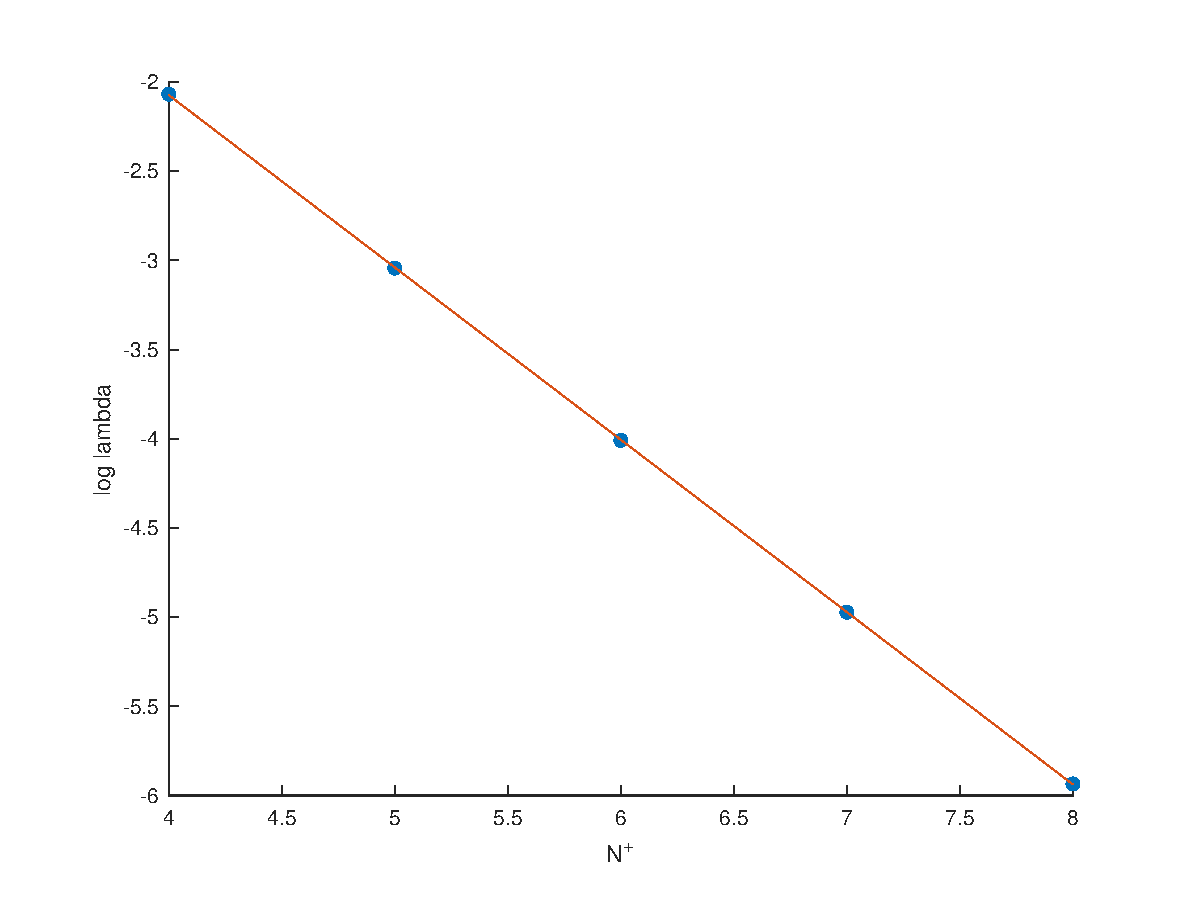
\includegraphics[width=10cm]{dnlslog.eps}
\label{fig:essspec1}
\caption{Stable double pulse}
\end{figure}

Slope of best-fit line is $-0.9660$, $\log \nu = -0.9206$, error is about $0.05$, which is great!


\section*{Lin for AL-dNLS}

Since we have two kernel eigenfunctions, we make the piecewise ansatz

\[
V_i^\pm(n) = d_i [ c_i S_1(n) + \tilde{S}_i^\pm(n) + \lambda(c_i T_1(n) + \tilde{T}_i^\pm(n))] + \tilde{d}_i [ c_i S_2(n) + \tilde{S}_i^\pm(n) + \lambda(c_i T_2(n) + \tilde{T}_i^\pm(n))]+ W_i^\pm(n)
\]

where we need better notation for the remainder terms, but you get the idea. Then for the jumps, we need to solve the jump equations in two directions, given by the two solutions to the adjoint problem.

\begin{align*}
Z_1 &= (0, 0, -\tilde{q}, q) \\
Z_2 &= (-\partial_\xi \tilde{q}, \partial_\xi q, 0, 0)
\end{align*}

The two Melnikov sums should be

\begin{align*}
M_1 &= \sum_j \langle Z_1(j+1), B T_1(j) \rangle = \sum_j q(j) q_\omega(j) \\
M_2 &= \sum_j \langle Z_2(j+1), B T_2(j) \rangle = \sum_j q(j) q_\omega(j) \\
\end{align*}

I think what happens is that, due to the structure (symplectic?) of AL-dNLS, the $Z_1$ and $Z_2$ jumps are, to leading order, independent from each other, so the jump equations become

\begin{align*}
\xi_i \approx c_{i+1} \langle Z_1(N_i^+), S_1(-N_i^-) \rangle (d_{i+1} - d_i)
+ c_{i-1} \langle Z_1(N_{i-1}^-), S_1(N_{i-1}^+) \rangle (d_i - d_{i-1}) - c_i \lambda M_1 \\
\tilde{\xi}_i \approx c_{i+1} \langle Z_2(N_i^+), S_2(-N_i^-) \rangle (\tilde{d}_{i+1} - \tilde{d}_i)
+ c_{i-1} \langle Z_2(N_{i-1}^-), S_2(N_{i-1}^+) \rangle (\tilde{d}_i - \tilde{d}_{i-1}) - c_i \lambda M_2
\end{align*}

\end{document}